\documentclass{article}
\usepackage{wasysym}
\usepackage{textcomp}
\usepackage{tikz}

\newcommand{\crel}{
	\hspace{-.6em}
	\begin{tikzpicture}[baseline={([yshift=-.8ex]current bounding box.center)}]
		\draw [->] (0,0) -- (0.45,0); 
		\draw [fill] (0.5,0) circle (0.05);
	\end{tikzpicture}
	\hspace{-.6em}
}

\newcommand{\rrel}{
	\hspace{-.6em}
	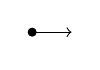
\begin{tikzpicture}[baseline={([yshift=-.8ex]current bounding box.center)}]
		\draw [fill] (0,0) circle (0.05);
		\draw [->] (0.05,0) -- (0.5,0);
	\end{tikzpicture}
	\hspace{-.6em}
}

\newcommand{\mrel}{
	\hspace{-.6em}
	\begin{tikzpicture}[baseline={([yshift=-.8ex]current bounding box.center)}]
		\draw [->] (0,0) -- (0.4,0);
		\draw (0.4,0) -- (0.475,0.075) -- (0.55,0) -- (0.475,-0.075) -- cycle;
	\end{tikzpicture}
	\hspace{-.6em}
}

\newcommand{\irel}{
	\hspace{-.6em}
	\begin{tikzpicture}[baseline={([yshift=-.8ex]current bounding box.center)}]
		\draw [->] (0,0) -- (0.4,0);
		\draw (0.41,0) -- (0.55,0);
		\draw (0.48,-0.07) -- (0.48, 0.07); 
	\end{tikzpicture}
	\hspace{-.6em}
}

\newcommand{\erel}{
	\hspace{-.6em}
	\begin{tikzpicture}[baseline={([yshift=-.8ex]current bounding box.center)}]
		\draw [->] (0,0) -- (0.4,0);
		\draw (0.41,0) -- (0.55,0);
		\draw (0.48, 0.05) circle (0.02);
		\draw (0.48, -0.05) circle (0.02); 
	\end{tikzpicture}
	\hspace{-.6em}
}

\begin{document}
	\section*{Problem}
	The system should support running a distributed DCR graph between multiple parties, under the assumption that any number of those parties will attempt to forge, collude, perjure or otherwise act maliciously, i. e. exhibiting byzantine failures.
	These distributed DCR graphs should always be accessible by all parties, connectivity permitting, and transparency must be ensured for all parties, in that they should always be aware of whether or not activities controlled by that party can be executed at any given time.

	% 1. There must be a happened-before relationship between the execution of an activity and the executions of its dependent activities % Studer Lamports FSM
	% 2. All serializations of the happened-before relationships must be valid execution sequences in DCR % Og opnå enighed om dem

	\section*{Definitions}
	\noindent
	Workflow: $G=(V,E)$ \\
	Activities: $V=\{v_1,\ \dots, v_n\}$ \\
	Activity States: $S=\{s_1,\ \dots, s_n\}$, where $s_i \subseteq \{Executed, Pending, Included\}$ corresponding to $V_i$.\\
	Relation: $R=($condition, response, milestone, include, exclude$)$, $e=(v_x, v_y, r_i)$, $E=\{e_1,\ \dots, e_m\}$\\
	Processes: $P =\{p_1,\ \dots, p_o\}$.\\
	History, $H_p(t)$: Sequence of activity executions up to, and at time $t$, as perceived by given process.\\
	Execution: $(v_i, t, p)$, where $v_i$ is the activity executed at time $t$, executed by process $p$.\\
	Dependant activities: An activity, $v_1$ is said to be dependant on another activity, $v_2$, when the DCR rules allowing $v_1$ to be executed, depends on the state of $v_2$. \\
	% Processor: $C$ is said to own a number of specific processes. Any process can only be owned by a single processor. \\
	% Activity responsibility: ... \\

	\section*{Requirements}
	\begin{description}
		\item[Consensus]:
			\begin{description}
				\item[Termination] Eventually each correct process sets its decision value (single activity state)
				\item[Partial agreement] % Decision vector = activity state
								Bottom is allowed as substitute for any activity state, unless that activity is owned by process or dependant on one such process. % Hvad er agreement
				\item[Integrity] If $p_i$ is correct, then all correct processes decide on $v_i$, or $\bot$ as the ith component of their vector. % Omformuler. Kan ikke genbruge i på den her måde
			\end{description}
		% \item[Concurrency]: DCR-rules for concurrency (only independent activities can be concurrent) (Tie-breaking). Nødvendig? Argumenter hvorfor Agreement + integrity giver concurrency løsning
		\item[Correctness]: Any state transition must be permitted by DCR logic or they will be rejected by correct nodes.
		\item[Non-repudiation]: $v_i$ must be provably proposed by $p_i$, within the bounds specified by any applied cryptography.
		% \item[Co-non-repudiation?]:
	\end{description}

	\section*{Scenarios} % Omformuleres til at bruge definitions.
	\begin{description}
		\item[Scenario 1] 
			$A\crel B$\\
			Alice must never decide $\bot$ for $A$. Bob must never decide $\bot$ for either $A$ or $B$.
		\item[Scenario 2]
			$A\crel B$, $A\crel C$\\
			Alice, Bob and Charlie must always decide the same value for $A$.\\
			Problem: Prevent Alice from telling Bob the state, but not Charlie. (Reduces to FLP.)
		\item[Scenario 3]
			$A\erel B$, $B\crel C$\\
			Alice and Bob must agree on the state of $A$, Bob and Charlie must agree on the state of $B$, only Charlie must agree on the value of $C$.
		\item[Scenario 4]
			$A\erel B$, $B\erel A$\\
			Both Alice and Bob must agree on both $A$ and $B$.\\
			Problem: Concurrency.
		\item[Scenario 5]
			$A\irel C$, $A\irel D$, $B\erel C$, $B\erel D$\\
			Both Alice and Bob must agree on only $A$ and $B$, respectively. Charlie must agree on everything except $D$, and Dahlia must agree on everything except $C$\\
			Problem: Concurrency (expanded), not serially equivalent if $C$ is included and $D$ is excluded after $A$ and $B$ have executed concurrently.			
	\end{description}


	\section*{Locking}
	
	\begin{description}
		\item[1: Exclude-include] $A \erel D, A \irel C, B \erel C, B \irel D$
		\item[2: Include condition] $A \irel C, C \crel B, B \irel D, D \crel A$ where $C$ and $D$ are excluded. 
		\item[3: Non-modifying to condition] $A \irel C, C \crel B, B \irel D, D \crel A$ where $D$ is excluded. 
	\end{description}

	\noindent There are three ways of locking when executing:

	\begin{description}
		\item[2 degrees back] has the disadvantage that notifications have to be pushed independently of locking. This locking does not work for graph 1, as A and B do not need to acquire locks on C and D. This means that the end state is subject to race conditions.
		\item[All adjacent] notifications need to be pushed in the second degree ocasionally (graph 2). 
		\item[2 degrees forward] has the inherent advantage of notifying relevant activities on execution. In graph 3, an execution of $A$ would only require locking on C, as opposed to the All adjacent locking scheme, which would require that D should be locked as well.
	\end{description}

	\section{The algorithm}
	Consider the events A, B and C, where A has relation AB to B, and B has relation BC to C.\\
	When A is executed:\\
	B must be locked if:\\
	AB is an effect (include, exclude, response)\\
	C must be locked if:\\
	AB is a constraining effect, and BC is a constraint (condition, milestone), in the following configuration:\\
	\begin{itemize}
		\item $A \irel B \crel C$ (B is excluded)
		\item $A \irel B \mrel C$ (B is excluded and pending)
		\item $A \rrel B \mrel C$ (B is not pending)
	\end{itemize}
\end{document}